


\tikzset{every picture/.style={line width=0.75pt}} %set default line width to 0.75pt        

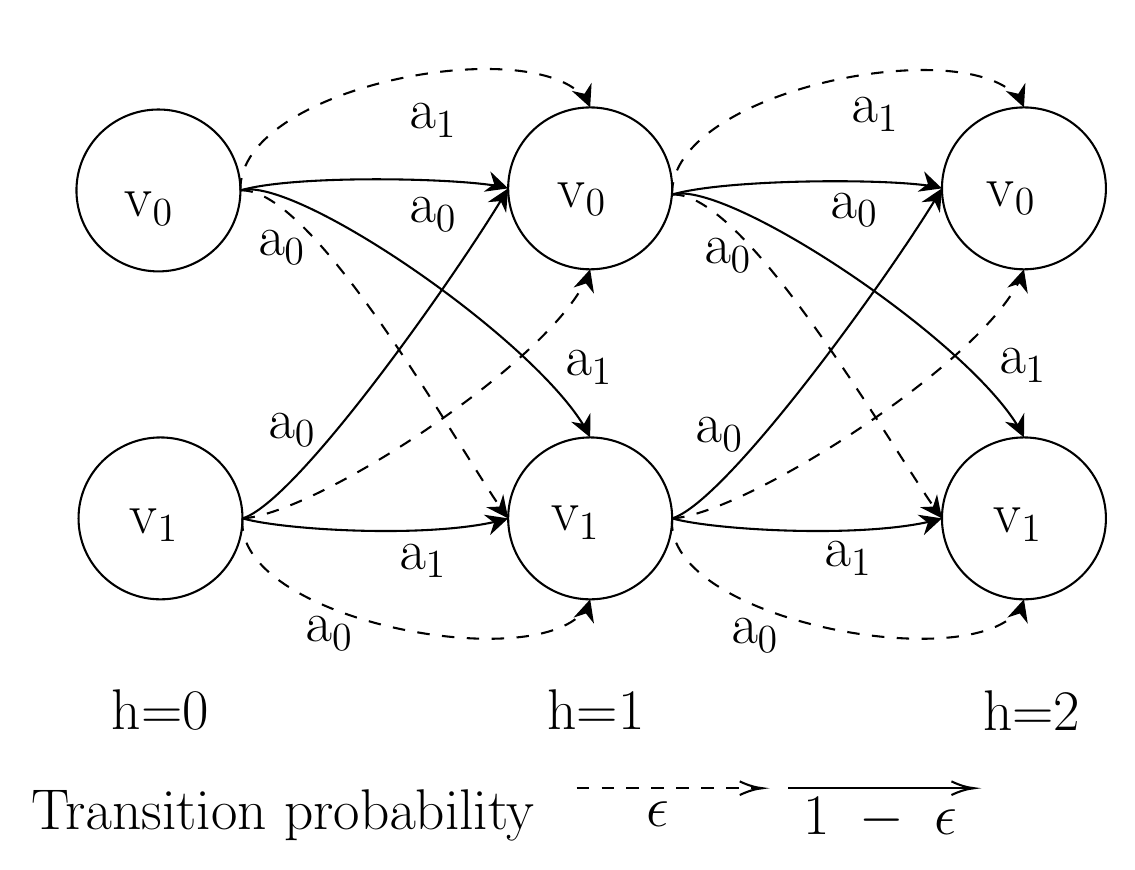
\begin{tikzpicture}[x=0.75pt,y=0.75pt,yscale=-1,xscale=1]
%uncomment if require: \path (0,1596); %set diagram left start at 0, and has height of 1596

%Shape: Ellipse [id:dp22781965006960792] 
\draw   (271,1256) .. controls (271,1234.46) and (288.68,1217) .. (310.5,1217) .. controls (332.32,1217) and (350,1234.46) .. (350,1256) .. controls (350,1277.54) and (332.32,1295) .. (310.5,1295) .. controls (288.68,1295) and (271,1277.54) .. (271,1256) -- cycle ;
%Shape: Ellipse [id:dp0009770034873839428] 
\draw   (270,1098) .. controls (270,1076.46) and (287.68,1059) .. (309.5,1059) .. controls (331.32,1059) and (349,1076.46) .. (349,1098) .. controls (349,1119.54) and (331.32,1137) .. (309.5,1137) .. controls (287.68,1137) and (270,1119.54) .. (270,1098) -- cycle ;
%Curve Lines [id:da7351476657211149] 
\draw    (349,1098) .. controls (374.18,1090.4) and (453.95,1091.83) .. (475.16,1096.27) ;
\draw [shift={(478,1097)}, rotate = 197.88] [fill={rgb, 255:red, 0; green, 0; blue, 0 }  ][line width=0.08]  [draw opacity=0] (10.72,-5.15) -- (0,0) -- (10.72,5.15) -- (7.12,0) -- cycle    ;
%Curve Lines [id:da9803616319422612] 
\draw  [dash pattern={on 4.5pt off 4.5pt}]  (350,1256) .. controls (385.77,1254.04) and (500.77,1179.09) .. (516.65,1138.44) ;
\draw [shift={(517.5,1136)}, rotate = 106.7] [fill={rgb, 255:red, 0; green, 0; blue, 0 }  ][line width=0.08]  [draw opacity=0] (10.72,-5.15) -- (0,0) -- (10.72,5.15) -- (7.12,0) -- cycle    ;
%Curve Lines [id:da6979473775260718] 
\draw  [dash pattern={on 4.5pt off 4.5pt}]  (349,1098) .. controls (384.59,1096.05) and (453.92,1222.43) .. (476.37,1253.78) ;
\draw [shift={(478,1256)}, rotate = 232.79] [fill={rgb, 255:red, 0; green, 0; blue, 0 }  ][line width=0.08]  [draw opacity=0] (10.72,-5.15) -- (0,0) -- (10.72,5.15) -- (7.12,0) -- cycle    ;
%Shape: Ellipse [id:dp4069934712250871] 
\draw   (478,1256) .. controls (478,1234.46) and (495.68,1217) .. (517.5,1217) .. controls (539.32,1217) and (557,1234.46) .. (557,1256) .. controls (557,1277.54) and (539.32,1295) .. (517.5,1295) .. controls (495.68,1295) and (478,1277.54) .. (478,1256) -- cycle ;
%Shape: Ellipse [id:dp5197280881747808] 
\draw   (478,1097) .. controls (478,1075.46) and (495.68,1058) .. (517.5,1058) .. controls (539.32,1058) and (557,1075.46) .. (557,1097) .. controls (557,1118.54) and (539.32,1136) .. (517.5,1136) .. controls (495.68,1136) and (478,1118.54) .. (478,1097) -- cycle ;
%Shape: Ellipse [id:dp9694823829725758] 
\draw   (687,1256) .. controls (687,1234.46) and (704.68,1217) .. (726.5,1217) .. controls (748.32,1217) and (766,1234.46) .. (766,1256) .. controls (766,1277.54) and (748.32,1295) .. (726.5,1295) .. controls (704.68,1295) and (687,1277.54) .. (687,1256) -- cycle ;
%Shape: Ellipse [id:dp47684208247159465] 
\draw   (687,1097) .. controls (687,1075.46) and (704.68,1058) .. (726.5,1058) .. controls (748.32,1058) and (766,1075.46) .. (766,1097) .. controls (766,1118.54) and (748.32,1136) .. (726.5,1136) .. controls (704.68,1136) and (687,1118.54) .. (687,1097) -- cycle ;
%Curve Lines [id:da8926054440407609] 
\draw    (350,1256) .. controls (375.97,1248.16) and (451.4,1141.4) .. (476.53,1099.48) ;
\draw [shift={(478,1097)}, rotate = 120.43] [fill={rgb, 255:red, 0; green, 0; blue, 0 }  ][line width=0.08]  [draw opacity=0] (10.72,-5.15) -- (0,0) -- (10.72,5.15) -- (7.12,0) -- cycle    ;
%Curve Lines [id:da6909503346391981] 
\draw    (350,1256) .. controls (370.96,1261.85) and (441.83,1265.8) .. (475.49,1256.72) ;
\draw [shift={(478,1256)}, rotate = 162.9] [fill={rgb, 255:red, 0; green, 0; blue, 0 }  ][line width=0.08]  [draw opacity=0] (10.72,-5.15) -- (0,0) -- (10.72,5.15) -- (7.12,0) -- cycle    ;
%Curve Lines [id:da4227819479888133] 
\draw  [dash pattern={on 4.5pt off 4.5pt}]  (350,1256) .. controls (345.59,1305.98) and (499.17,1333.87) .. (516.6,1297.32) ;
\draw [shift={(517.5,1295)}, rotate = 106.7] [fill={rgb, 255:red, 0; green, 0; blue, 0 }  ][line width=0.08]  [draw opacity=0] (10.72,-5.15) -- (0,0) -- (10.72,5.15) -- (7.12,0) -- cycle    ;
%Curve Lines [id:da43040746641683647] 
\draw  [dash pattern={on 4.5pt off 4.5pt}]  (349,1098) .. controls (347.53,1047.04) and (495.4,1020.09) .. (516.38,1055.74) ;
\draw [shift={(517.5,1058)}, rotate = 247.69] [fill={rgb, 255:red, 0; green, 0; blue, 0 }  ][line width=0.08]  [draw opacity=0] (10.72,-5.15) -- (0,0) -- (10.72,5.15) -- (7.12,0) -- cycle    ;
%Curve Lines [id:da2169138512030282] 
\draw    (349,1098) .. controls (374.97,1090.16) and (492.66,1170.68) .. (516.18,1214.37) ;
\draw [shift={(517.5,1217)}, rotate = 245.06] [fill={rgb, 255:red, 0; green, 0; blue, 0 }  ][line width=0.08]  [draw opacity=0] (10.72,-5.15) -- (0,0) -- (10.72,5.15) -- (7.12,0) -- cycle    ;
%Curve Lines [id:da6364602537352781] 
\draw    (557,1100) .. controls (582.18,1092.4) and (662.85,1092.02) .. (684.15,1096.29) ;
\draw [shift={(687,1097)}, rotate = 197.88] [fill={rgb, 255:red, 0; green, 0; blue, 0 }  ][line width=0.08]  [draw opacity=0] (10.72,-5.15) -- (0,0) -- (10.72,5.15) -- (7.12,0) -- cycle    ;
%Curve Lines [id:da33346792042439244] 
\draw  [dash pattern={on 4.5pt off 4.5pt}]  (557,1256) .. controls (592.77,1254.04) and (709.69,1179.09) .. (725.65,1138.44) ;
\draw [shift={(726.5,1136)}, rotate = 106.7] [fill={rgb, 255:red, 0; green, 0; blue, 0 }  ][line width=0.08]  [draw opacity=0] (10.72,-5.15) -- (0,0) -- (10.72,5.15) -- (7.12,0) -- cycle    ;
%Curve Lines [id:da9081851392102287] 
\draw  [dash pattern={on 4.5pt off 4.5pt}]  (557,1100) .. controls (592.59,1098.05) and (662.87,1222.53) .. (685.37,1253.78) ;
\draw [shift={(687,1256)}, rotate = 232.79] [fill={rgb, 255:red, 0; green, 0; blue, 0 }  ][line width=0.08]  [draw opacity=0] (10.72,-5.15) -- (0,0) -- (10.72,5.15) -- (7.12,0) -- cycle    ;
%Curve Lines [id:da22645110117463774] 
\draw    (557,1256) .. controls (582.97,1248.16) and (660.32,1141.4) .. (685.52,1099.48) ;
\draw [shift={(687,1097)}, rotate = 120.43] [fill={rgb, 255:red, 0; green, 0; blue, 0 }  ][line width=0.08]  [draw opacity=0] (10.72,-5.15) -- (0,0) -- (10.72,5.15) -- (7.12,0) -- cycle    ;
%Curve Lines [id:da8221163768033788] 
\draw    (557,1256) .. controls (577.96,1261.85) and (650.73,1265.8) .. (684.48,1256.72) ;
\draw [shift={(687,1256)}, rotate = 162.9] [fill={rgb, 255:red, 0; green, 0; blue, 0 }  ][line width=0.08]  [draw opacity=0] (10.72,-5.15) -- (0,0) -- (10.72,5.15) -- (7.12,0) -- cycle    ;
%Curve Lines [id:da22332666192427086] 
\draw  [dash pattern={on 4.5pt off 4.5pt}]  (557,1256) .. controls (552.59,1305.98) and (708.09,1333.87) .. (725.6,1297.32) ;
\draw [shift={(726.5,1295)}, rotate = 106.7] [fill={rgb, 255:red, 0; green, 0; blue, 0 }  ][line width=0.08]  [draw opacity=0] (10.72,-5.15) -- (0,0) -- (10.72,5.15) -- (7.12,0) -- cycle    ;
%Curve Lines [id:da015628806951311303] 
\draw  [dash pattern={on 4.5pt off 4.5pt}]  (557,1100) .. controls (555.53,1049.04) and (704.36,1020.17) .. (725.38,1055.74) ;
\draw [shift={(726.5,1058)}, rotate = 247.69] [fill={rgb, 255:red, 0; green, 0; blue, 0 }  ][line width=0.08]  [draw opacity=0] (10.72,-5.15) -- (0,0) -- (10.72,5.15) -- (7.12,0) -- cycle    ;
%Curve Lines [id:da09275044993717585] 
\draw    (557,1100) .. controls (582.97,1092.16) and (701.62,1170.76) .. (725.18,1214.37) ;
\draw [shift={(726.5,1217)}, rotate = 245.06] [fill={rgb, 255:red, 0; green, 0; blue, 0 }  ][line width=0.08]  [draw opacity=0] (10.72,-5.15) -- (0,0) -- (10.72,5.15) -- (7.12,0) -- cycle    ;
%Straight Lines [id:da0927494444452106] 
\draw  [dash pattern={on 4.5pt off 4.5pt}]  (511,1386) -- (598.5,1386) ;
\draw [shift={(600.5,1386)}, rotate = 180] [color={rgb, 255:red, 0; green, 0; blue, 0 }  ][line width=0.75]    (10.93,-3.29) .. controls (6.95,-1.4) and (3.31,-0.3) .. (0,0) .. controls (3.31,0.3) and (6.95,1.4) .. (10.93,3.29)   ;
%Straight Lines [id:da08454871327533309] 
\draw    (613,1386) -- (700.5,1386) ;
\draw [shift={(702.5,1386)}, rotate = 180] [color={rgb, 255:red, 0; green, 0; blue, 0 }  ][line width=0.75]    (10.93,-3.29) .. controls (6.95,-1.4) and (3.31,-0.3) .. (0,0) .. controls (3.31,0.3) and (6.95,1.4) .. (10.93,3.29)   ;

% Text Node
\draw (247,1385) node [anchor=north west][inner sep=0.75pt]  [font=\huge] [align=left] {Transition probability};
% Text Node
\draw (356,1116) node [anchor=north west][inner sep=0.75pt]  [font=\huge] [align=left] {a\textsubscript{0}};
% Text Node
\draw (567,1206) node [anchor=north west][inner sep=0.75pt]  [font=\huge] [align=left] {a\textsubscript{0}};
% Text Node
\draw (543,1391) node [anchor=north west][inner sep=0.75pt]  [font=\huge] [align=left] { $\displaystyle \epsilon $};
% Text Node
\draw (618.75,1389) node [anchor=north west][inner sep=0.75pt]  [font=\huge] [align=left] { $\displaystyle 1\ -\ \epsilon $};
% Text Node
\draw (429,1100) node [anchor=north west][inner sep=0.75pt]  [font=\huge] [align=left] {a\textsubscript{0}};
% Text Node
\draw (361,1204) node [anchor=north west][inner sep=0.75pt]  [font=\huge] [align=left] {a\textsubscript{0}};
% Text Node
\draw (424,1267) node [anchor=north west][inner sep=0.75pt]  [font=\huge] [align=left] {a\textsubscript{1}};
% Text Node
\draw (710.4,1249.6) node [anchor=north west][inner sep=0.75pt]  [font=\huge] [align=left] {v\textsubscript{1}};
% Text Node
\draw (504,1174) node [anchor=north west][inner sep=0.75pt]  [font=\huge] [align=left] {a\textsubscript{1}};
% Text Node
\draw (379,1302) node [anchor=north west][inner sep=0.75pt]  [font=\huge] [align=left] {a\textsubscript{0}};
% Text Node
\draw (429,1055) node [anchor=north west][inner sep=0.75pt]  [font=\huge] [align=left] {a\textsubscript{1}};
% Text Node
\draw (497.2,1248.6) node [anchor=north west][inner sep=0.75pt]  [font=\huge] [align=left] {v\textsubscript{1}};
% Text Node
\draw (294.2,1249.8) node [anchor=north west][inner sep=0.75pt]  [font=\huge] [align=left] {v\textsubscript{1}};
% Text Node
\draw (707.2,1092.2) node [anchor=north west][inner sep=0.75pt]  [font=\huge] [align=left] {v\textsubscript{0}};
% Text Node
\draw (500.4,1092.6) node [anchor=north west][inner sep=0.75pt]  [font=\huge] [align=left] {v\textsubscript{0}};
% Text Node
\draw (291.8,1097.2) node [anchor=north west][inner sep=0.75pt]  [font=\huge] [align=left] {v\textsubscript{0}};
% Text Node
\draw (632,1098) node [anchor=north west][inner sep=0.75pt]  [font=\huge] [align=left] {a\textsubscript{0}};
% Text Node
\draw (629,1266) node [anchor=north west][inner sep=0.75pt]  [font=\huge] [align=left] {a\textsubscript{1}};
% Text Node
\draw (571,1120) node [anchor=north west][inner sep=0.75pt]  [font=\huge] [align=left] {a\textsubscript{0}};
% Text Node
\draw (584,1303) node [anchor=north west][inner sep=0.75pt]  [font=\huge] [align=left] {a\textsubscript{0}};
% Text Node
\draw (642,1052) node [anchor=north west][inner sep=0.75pt]  [font=\huge] [align=left] {a\textsubscript{1}};
% Text Node
\draw (285.6,1336.8) node [anchor=north west][inner sep=0.75pt]  [font=\huge] [align=left] {h=0};
% Text Node
\draw (705.4,1337.4) node [anchor=north west][inner sep=0.75pt]  [font=\huge] [align=left] {h=2};
% Text Node
\draw (495.4,1336.8) node [anchor=north west][inner sep=0.75pt]  [font=\huge] [align=left] {h=1};
% Text Node
\draw (713,1173) node [anchor=north west][inner sep=0.75pt]  [font=\huge] [align=left] {a\textsubscript{1}};


\end{tikzpicture}